\newpage
\section{Builder Pattern}

Builder pattern builds a complex object using simple objects and using a step by step approach. This type of design pattern comes under creational pattern as this pattern provides one of the best ways to create an object.
A Builder class builds the final object step by step. This builder is independent of other objects.

\subsection{Class Diagram}

\begin{figure}[h]
\centering
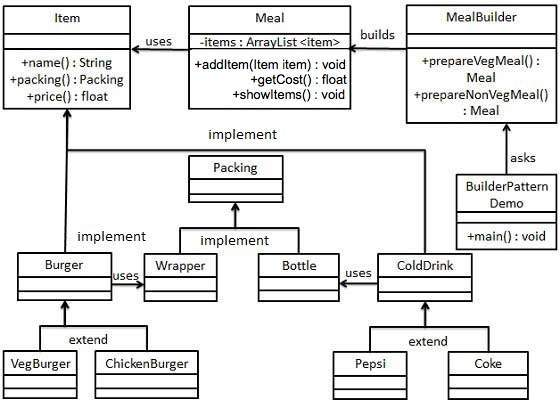
\includegraphics[scale=0.5]{builder}
\caption{Class Diagram of Builder Pattern}
\end{figure}

\newpage
\subsection{Source Code (Java)}

\subsubsection{Item Interface}

\begin{minted}{java}
public interface Item {
   public String name();
   public Packing packing();
   public float price();	
}
\end{minted}

\subsubsection{Packing Interface}

\begin{minted}{java}
public interface Packing {
   public String pack();
}
\end{minted}

\subsubsection{Wrapper Class}

\begin{minted}{java}
public class Wrapper implements Packing {

   @Override
   public String pack() {
      return "Wrapper";
   }
}
\end{minted}

\subsubsection{Bottle Class}

\begin{minted}{java}
public class Bottle implements Packing {

   @Override
   public String pack() {
      return "Bottle";
   }
}
\end{minted}

\subsubsection{Burger abstract Class}

\begin{minted}{java}
public abstract class Burger implements Item {

   @Override
   public Packing packing() {
      return new Wrapper();
   }

   @Override
   public abstract float price();
}
\end{minted}

\subsubsection{ColdDrink abstract Class}

\begin{minted}{java}
public abstract class ColdDrink implements Item {

	@Override
	public Packing packing() {
       return new Bottle();
	}

	@Override
	public abstract float price();
}
\end{minted}

\subsubsection{VegBurger Class}

\begin{minted}{java}
public class VegBurger extends Burger {

   @Override
   public float price() {
      return 25.0f;
   }

   @Override
   public String name() {
      return "Veg Burger";
   }
}
\end{minted}

\subsubsection{ChickenBurger Class}

\begin{minted}{java}
public class ChickenBurger extends Burger {

   @Override
   public float price() {
      return 50.5f;
   }

   @Override
   public String name() {
      return "Chicken Burger";
   }
}
\end{minted}

\subsubsection{Coke Class}

\begin{minted}{java}
public class Coke extends ColdDrink {

   @Override
   public float price() {
      return 30.0f;
   }

   @Override
   public String name() {
      return "Coke";
   }
}
\end{minted}

\subsubsection{Pepsi Class}

\begin{minted}{java}
public class Pepsi extends ColdDrink {

   @Override
   public float price() {
      return 35.0f;
   }

   @Override
   public String name() {
      return "Pepsi";
   }
}
\end{minted}

\subsubsection{Meal Class}

\begin{minted}{java}
import java.util.ArrayList;
import java.util.List;

public class Meal {
   private List<Item> items = new ArrayList<Item>();	

   public void addItem(Item item){
      items.add(item);
   }

   public float getCost(){
      float cost = 0.0f;
      
      for (Item item : items) {
         cost += item.price();
      }		
      return cost;
   }

   public void showItems(){
   
      for (Item item : items) {
         System.out.print("Item : " + item.name());
         System.out.print(", Packing : " + item.packing().pack());
         System.out.println(", Price : " + item.price());
      }		
   }	
}
\end{minted}

\subsubsection{MealBuilder Class}

\begin{minted}{java}
public class MealBuilder {

   public Meal prepareVegMeal (){
      Meal meal = new Meal();
      meal.addItem(new VegBurger());
      meal.addItem(new Coke());
      return meal;
   }   

   public Meal prepareNonVegMeal (){
      Meal meal = new Meal();
      meal.addItem(new ChickenBurger());
      meal.addItem(new Pepsi());
      return meal;
   }
}
\end{minted}

\subsubsection{Driver Class}

\begin{minted}{java}
public class BuilderPatternDemo {
   public static void main(String[] args) {
   
      MealBuilder mealBuilder = new MealBuilder();

      Meal vegMeal = mealBuilder.prepareVegMeal();
      System.out.println("Veg Meal");
      vegMeal.showItems();
      System.out.println("Total Cost: " + vegMeal.getCost());

      Meal nonVegMeal = mealBuilder.prepareNonVegMeal();
      System.out.println("\n\nNon-Veg Meal");
      nonVegMeal.showItems();
      System.out.println("Total Cost: " + nonVegMeal.getCost());
   }
}
\end{minted}

\subsection{Output}

\begin{minted}{text}
Veg Meal
Item : Veg Burger, Packing : Wrapper, Price : 25.0
Item : Coke, Packing : Bottle, Price : 30.0
Total Cost: 55.0


Non-Veg Meal
Item : Chicken Burger, Packing : Wrapper, Price : 50.5
Item : Pepsi, Packing : Bottle, Price : 35.0
Total Cost: 85.5
\end{minted}